% Copyright 2015 Daniel Nikpayuk
\documentclass[twoside]{article}
\usepackage[letterpaper,left=1cm,right=1cm,top=2cm,bottom=2cm]{geometry}
\usepackage{amsmath}
\usepackage{amsfonts}
\usepackage{graphicx}
\usepackage{hyperref}
\usepackage{xcolor}
\usepackage{bm}

\newcommand{\st}{$ ^{\mbox{\scriptsize st}} $ }
\newcommand{\nd}{$ ^{\mbox{\scriptsize nd}} $ }
\newcommand{\rd}{$ ^{\mbox{\scriptsize rd}} $ }

\renewcommand{\th}{$ ^{\mbox{\scriptsize th}} $ }
%\th command exists, it gives the old english symbol used for `theta' IPA (voiceless)

\renewcommand{\leq}{\ensuremath{\quad\le\qquad}}
\renewcommand{\geq}{\ensuremath{\quad\ge\qquad}}

\newcommand{\seq}[1][u]{\ensuremath{<\!#1\!>}}
\newcommand{\bseq}[1][u]{\ensuremath{<\!\!\bm{#1}\!\!>}}
\newcommand{\underseq}[2][u]{\ensuremath{\underset{#2}{<\!#1\!>}}}
\newcommand{\bunderseq}[2][u]{\ensuremath{\underset{#2}{<\!\!\bm{#1}\!\!>}}}

\newcommand{\radix}[2][u]{\ensuremath{\underset{#2}{(#1)}}}
\newcommand{\radixp}[3][u]{\ensuremath{\underset{#2}{(#1)^{#3}}}}
\newcommand{\bradix}[2][u]{\ensuremath{\underset{#2}{(\bm{#1})}}}
\newcommand{\bradixp}[3][u]{\ensuremath{\underset{#2}{(\bm{#1})^{#3}}}}

\newcommand{\numer}[3][w]{\ensuremath{(\bm{#1})_{#2\le k\le #3}}}
\newcommand{\denom}[3][y]{\ensuremath{(\bm{#1})_{#2\le k <  #3}}}

\newcommand{\ldiv}[1]{\ensuremath{\raisebox{0.045em}{)}\hspace{-0.3275em}\overline{\ #1}}}

\newtheorem{theorem}{Theorem}[section]
\newtheorem{lemma}{Lemma}[section]
\newtheorem{corollary}[theorem]{Corollary}

\newenvironment{proof}[1][Proof]{\begin{trivlist}
\item[\hskip \labelsep {\bfseries #1}]}{\end{trivlist}}
\newenvironment{definition}[1][Definition]{\begin{trivlist}
\item[\hskip \labelsep {\bfseries Definition (#1):}]}{\end{trivlist}}

\newcommand{\qed}{\nobreak \ifvmode \relax \else
      \ifdim\lastskip<1.5em \hskip-\lastskip
      \hskip1.5em plus0em minus0.5em \fi \nobreak
      \vrule height0.5em width0.5em depth0.25em\fi}

\newcounter{equationcount}
\newcommand{\eqncount}{\refstepcounter{equationcount}\qquad (\theequationcount)}

\pagestyle{empty}
\begin{document}

\begin{figure}[h]
\centering

\includegraphics[width=1in]{cc-by-nc.png}\\[0.1in]
\tiny This article is licensed under \\
\href{http://creativecommons.org/licenses/by-nc/4.0/}
{Creative Commons Attribution-NonCommercial 4.0 International.}\\[0.3in]
\end{figure}

This article provides an exposition---with an original proof---of the computationally optimized \emph{division}
algorithm discussed in Donald Knuth's ``The Art of Computer Programming Volume 2'', in particular: ``Chapter 4---Arithmetic,
4.3.1 The Classical Algorithms''.  If Knuth has already put in the work, why revisit this topic?

\begin{enumerate}
\item Knuth's classic textbook is under copyright and it is surprisingly just about impossible to find digital copies to
	it or any derivative work for quick reference.
\item Knuth's proof is only partial, leaving the gaps as exercises. Math and computation require rigour---especially
	for such a fundamental routine as division.
\item Knuth's proof uses some old assembly language which is pretty much unreadable to anyone but historians of programming.
	Although I do not include any code from any specific language here, the optimized division algorithm proven will be
	used toward a C++ template implementation.
\item Knuth's proof uses---in my opinion---ad-hoc inequality manipulations. It is often the case in the history of mathematical
	proofs, that what matters most is a fast proof, and because of that the very first proof given tends to be messy.
	Regardless, a lot of time has passed and we have better notation and theories. It is always worth revisiting messy
	ugly proofs and coming up with shorter, cleaner, narrative proofs which aid the mathematician in furthering her skill-set.
	With the exception of \emph{the first}, a proof isn't of much use unless it furthers your ability to think in new ways.
	Surprisingly---given all he's done for math---Knuth's proof misses the mark in this regard.
\end{enumerate}

The exposition given here is intended to be thorough but educational. I tend to include and show far more steps in my derivations
than is otherwise required when proof-writing for other mathematicians. The idea is to illustrate general strategies of inequality
manipulation for use beyond the direct application given here. This is most useful for those who may lack the necessary background.
For instance, having taken honours math myself I have previously learned many tricks when it comes to inequality manipulations of
Weierstrass' \emph{epsilons} and \emph{deltas}, but even then I was surprised to discover new ways of looking at very basic inequality
arithmetic not yet seen in my rigourous education.

As it turns out, the implementation of multiple precision long division is rather involved for an otherwise conceptually simple
algorithm. We will break it down by complexity.

\section*{Intuitive long division}

Let's start with a simple division:
$$ 9\ldiv{200} $$

Back to our school days---before calculators---we notice our \emph{divisor} is only a single digit (the digit `$ 9 $'),
and so we start by comparing single digits in our \emph{dividend}: $ 200 $. Our first digit is $ 2 $ which is too small
($ 9\not\le 2 $), and so we continue by appending the next digit which works ($ 9\le 20 $). By memory we know that
$ 20\div 9 = 2 $, and so we can append our first digit of the \emph{quotient}:

$$ \begin{array}{rr}
2\hspace{0.075em}\_	\\
9\ldiv{200}		\\
\end{array} $$
with the underscore `$ \_ $' indicating the expected and remaining but yet-to-be-determined digit. We multiply our found
digit and subtract from the lead of the dividend, providing us with a \emph{remainder} as seed for our recursive algorithm:

$$ \begin{array}{rr}
2\hspace{0.075em}\_		\\
9\ldiv{200}			\\
\underline{18\hspace{0.175em}}\	\\
2\hspace{0.175em}\ 
\end{array} $$

\newpage

we then bring down the next digits as needed---or \emph{all} remaining digits,
to conceptually simplify the iterative step---and repeat:

$$ \begin{array}{rcrcr}
2\hspace{0.075em}\_		&	&		&	& 22					\\
9\ldiv{200}			& \to	& 9\ldiv{20}	& \to	& 9\ldiv{200}				\\
\underline{18\hspace{0.175em}}\	&	&		&	& \underline{18\hspace{0.175em}}\	\\
20				&	&		&	& 20					\\
				&	&		&	& \underline{18}			\\
				&	&		&	& 2					\\
\end{array} $$

\section*{Single-digit division}

Single digit division is done in the sense that the divisor has a single digit with respect to the base.
The above example has base $ 10 $ and it is a single digit division, the divisor being $ 9 $.

In practice, in implementing toward computational division, we frankly want to use as large a base as possible
with respect to the \emph{register} size. The reason being is that an \emph{optimized} algorithm and an \emph{efficient}
algorithm aren't always necessarily the same thing. Computer processors have basic algorithms like addition, subtraction,
multiplication and division hardcoded within their circuits, and hardware runtimes are always orders of magnitude faster
than software simulations of hardware circuits. So for example, if we're working with a $ 64 $-bit architecture, it means
we'd ideally like our \emph{multiple precision} base to be $ 2^{64} $ \emph{itself} with our software division algorithm
optimized toward using the hardware division circuits as much as possible with few simulated softward division calculations.

\begin{quote}
\em
Before going on, I would like to make it clear this section presents an inefficient approach to solving the
single-digit division algorithm. The reason I present it at all is that it is the best example I could come
up with of a {\bfseries direct approach}---the point being that if the best direct approach is known to be
inefficient, we have to start looking for indirect approaches, in particular: approximation methods.  I present
this section for educational purposes.  As for the efficient approach, the theory behind the multiple-digit division
algorithm presented in the following section can be used to implement such a single-digit version in practice.
\end{quote}

In the regard that we are privileging use of hardware division, and assuming our base is effectively the register size,
it means we can't actually represent the base itself with the registers. Although you could consider this a very serious
problem, we do in fact have a way around this: We can still represent $ b-1 $, and furthermore the number theoretic division
theorem tells us:
$$ b-1=qd+r,\qquad 0\le r < d $$
where $ d $ is the divisor, and $ q,r $ are unique integers. This implies:
$$ b=qd+r+1 $$
with two possible cases: $ r+1=d $ or $ r+1 < d $. In the case that $ r+1=d $ we have:
$$ \begin{array}{rcl}
b	& = &	qd+r+1	\\
	& = &	qd+d	\\
	& = &	(q+1)d	\\
\end{array} $$
while in the case that $ r+1 < d $ we can simply leave it as $ b=qd+r+1 $. You might protest saying: ``How can we know
for sure that $ q $ or $ q+1 $ are representable? (less than the base)'' to which I would say in the case that
our divisor $ d=1 $ we should optimize and skip the calculation and simply return the dividend which then leaves
the case that $ d > 1 $; it is easy to show then that $ q,q+1 < b $.

Being able to divide the base itself is significant because if you've noticed in our intuitive division example above,
there are two possible cases: The dividend digit we're testing is greater than or equal to our divisor and so we compute
single digit divided-by single digit division---which we assume our hardware is able to handle all on its own---or we have
to add a second digit to complete the iterative division step; in which case if our base equals the register size we have
no automatic hardware division primitives to work with directly. In the latter case, we would represent two digits from
the dividend as such:
$$ (n_1n_0)_b\quad:=\quad n_1b+n_0,\qquad 0\le n_1,n_0 < b $$
Our implementation must be able to handle this case.\footnote{I should mention there is a second possible implementation:
We choose our base to be the square root of the register size (for example if our register size is $ 64 $-bit our
base would be $ 2^{32} $. In such an implementation, we can then use the hardware circuit division in both cases.
The tradeoff is the \emph{array} size effectively doubles, and there is some deadweight loss in terms of register
calculations.} Given our above decomposition of the base, from this viewpoint we now have:
$$ \begin{array}{rclcl}
b		& = &	(q+1)d		& \mbox{or} &	qd+r+1			\\
n_1b		& = &	(n_1(q+1))d	& \mbox{or} &	(n_1q)d+n_1(r+1)	\\
n_1b+n_0	& = &	(n_1(q+1))d+n_0	& \mbox{or} &	(n_1q)d+n_1(r+1)+n_0	\\
(n_1n_0)_b	& = &	(n_1(q+1))d+n_0	& \mbox{or} &	(n_1q)d+n_1(r+1)+n_0	\\
\end{array} $$

Let's clean this up a bit first by standardizing our notation: Let $ n\oslash d $ denote the unique quotient guaranteed
by the division-remainder theorem, with $ n\ominus d $ as unique remainder. With this, our specific $ q,r $---within this
new notation---are now short-form for:
$$ \begin{array}{rcl}
q	& := &	(b-1)\oslash d	\\
r	& := &	(b-1)\ominus d	\\
\end{array} $$

Regardless, in the first case above we now have:
$$ \begin{array}{rcl}
(n_1n_0)_b\oslash d	& = &	n_1(q+1)+n_0\oslash d	\\
(n_1n_0)_b\ominus d	& = &	n_0\ominus d		\\
\end{array} $$
and in the second case we otherwise have
$$ \begin{array}{rcl}
(n_1n_0)_b\oslash d	& = &	n_1q+(n_1(r+1)+n_0)\oslash d	\\
(n_1n_0)_b\ominus d	& = &	(n_1(r+1)+n_0)\ominus d		\\
\end{array} $$
but the current form of this second case is currently problematic as we may not know how to compute
$ (m+n)\oslash d $ for arbitrary $ m,n $.  The answer in fact comes from the following distributive law:
\begin{lemma}
$$ \begin{array}{rcl}
(m+n)\oslash d & = & m\oslash d+n\oslash d+(m\ominus d+n\ominus d)\oslash d \\
(m+n)\ominus d & = & (m\ominus d+n\ominus d)\ominus d
\end{array} $$
\end{lemma}

\begin{proof}
We first decompose:
$$ \begin{array}{rclcl}
m & = & q_md+r_m & , & 0\le r_m < d \\
n & = & q_nd+r_n & , & 0\le r_n < d \\
\end{array} $$
then add:
$$ \begin{array}{rcl}
m+n	& = & (q_md+r_m)+(q_nd+r_n) \\
	& = & (q_m+q_n)d+(r_m+r_n) \\
\end{array} $$
which may be in the ideal form for a decomposition, but it may not meet the expected constraint that $ 0\le r_m+r_n < d $.
In fact the best we can say is $ 0\le r_m+r_n < 2d $. Thus our decomposition necessarily becomes:
$$ \begin{array}{rcl}
(m+n)\oslash d & = & m\oslash d+n\oslash d+(m\ominus d+n\ominus d)\oslash d	\\
(m+n)\ominus d & = & (m\ominus d+n\ominus d)\ominus d\quad\qed
\end{array} $$

\end{proof}
This leads us to our expanded (more complicated) second form of our second case:
$$ \begin{array}{rcl}
(n_1n_0)_b\oslash d	& = & n_1q+n_1(r+1)\oslash d+n_0\oslash d+(n_1(r+1)\ominus d+n_0\ominus d)\oslash d	\\
(n_1n_0)_b\ominus d	& = & (n_1(r+1)\ominus d+n_0\ominus d)\ominus d	\\
\end{array} $$

Finally, this is where we run into our computational inefficiency with this direct approach:  In the case
$$ (n_1n_0)_b\oslash d\quad=\quad n_1q+n_1(r+1)\oslash d+n_0\oslash d+(n_1(r+1)\ominus d+n_0\ominus d)\oslash d $$
we have a practical problem as the $ n_1(r+1) $ term may be larger than $ b $ (overflow in b).
We note by assumption that $ r+1 < d $.  As well, in this special case we also know that $ n_1 < d $---as we would
otherwise not be working with two digits at all. As $ d $ is in the open range $ (0, b) $ we can't ignore the possibility
that $ b < n_1(r+1) < b^2 $, in which case we'd need two digits to represent this number---and in such a case it seems
like we're back where we started: A two digit number which we need to divide by $ d $.

The first conclusion we can draw from is in knowing that the general division algorithm itself will halt; thus we start
with
$$ n_1b+n_0 $$
and in the process---in the worse case scenario---return to a new two digit number as follows:
$$ m_1b+m_0\quad:=\quad n_1(r+1) $$
Let's recontextualize and restate this in more recursive notation: We start with
$$ n_1^{(0)}b+n_0^{(0)} $$
and end up with
$$ n_1^{(1)}b+n_0^{(1)}\quad:=\quad n_1^{(0)}(r+1) $$
In a streamlined understanding, our recursive loop would play out as follows:
$$ n_1^{(0)}\quad\to\quad n_1^{(1)}\quad\to\quad\ldots\quad\to\quad n_1^{(k)}=0 $$
where we would reach some iteration $ k $ such that our $ n_1^{(k)}=0 $, and thus the loop would halt. We'd still have some
other computations to make to finish things up, but they would be outside the loop itself.

Let's analyse this loop a bit more closely. Notice each following
leading digits $ n_1^{(j)} $ can be defined from the previous as
$$ n_1^{(j)}=n_1^{(j-1)}(r+1)\oslash b $$
and we also happen to know (from the quotient-remainder theorem) that our quotient satisfies the following inequality:
$$ \frac{n_1^{(j-1)}(r+1)}{b}-1\quad <\qquad n_1^{(j)} $$
which if we rearrange and clean up a little we get
$$ n_1^{(j)}\quad >\qquad -1+\frac{(r+1)}{b}n_1^{(j-1)} $$
which if you recursively expand (by means of the transitive law), you get
$$ n_1^{(j)}\quad >\qquad \sum_{0\le i < s}(-1)\left(\frac{r+1}{b}\right)^i+\left(\frac{r+1}{b}\right)^s n_1^{(j-s)} $$
which can be proven with mathematical induction to be true for $ s\ge 1 $. In anycase, by setting $ s:=j $ we have
$$ n_1^{(j)}\quad >\qquad -\sum_{0\le i < j}\left(\frac{r+1}{b}\right)^i+\left(\frac{r+1}{b}\right)^j n_1^{(0)} $$
and by setting $ j:=k $ where we know our loop halts, we have
$$ 0\quad >\qquad -\sum_{0\le i < k}\left(\frac{r+1}{b}\right)^i+\left(\frac{r+1}{b}\right)^k n_1^{(0)} $$
but let's notationally simplify this relation by conventionally setting $ c:=\frac{r+1}{b} $ so that
$$ 0\quad >\qquad -\sum_{0\le i < k}c^i+c^k n_1^{(0)} $$
which when remembering our $ n_1^{(0)} $ is just fancy talk for our original $ n_1 $ simplifies to
$$ \sum_{0\le i < k}c^i\quad >\qquad c^k n_1 $$
of course we can simplify a bit further still with the basic geometric series
$$ \frac{1-c^k}{1-c}\quad >\qquad c^k n_1 $$

At this point we are now interested in isolating $ k $ as we want to know how many loops we need to run:
$$ 1-c^k\quad >\qquad (1-c)c^k n_1 $$
which when rearranged we get
$$ 1\quad >\qquad c^k(1+(1-c)n_1) $$
$$ 1+(1-c)n_1\quad <\qquad (c^{-1})^k $$
notice our $ c^{-1}=\left(\frac{b}{r+1}\right) $ is such that $ c^{-1} > 1 $,
and so taking the logarithm under it preserves our ordering relation
$$ log_{c^{-1}}(1+(1-c)n_1)\quad <\qquad k $$
thus, regardless of what our $ r $ turns out to be, as our $ n_1 $ grows larger so does the number of cycles of our loop.
In particular, if our $ r $ does turn out to be quite small, and our divisor $ d $ (and thus the potential of $ n_1 $)
are known to be quite large, this algorithm requires more and more steps in the loop before it halts.

Such a direct approach algorithm is heuristic: In the best case scenario, it does quite well in fact, but in the worse,
it's not at all practical.

Given the operation of division is \emph{critical infrastructure} when it comes to the world of computing, we have shown
we need a better---and in this case an indirect---approach for our single-digit divisor division algorithm:
The treatment of such is overall given in what follows.

\section*{Multiple-digit division}

The case of multiple-digit division is in fact the same algorithm, but there are complications of efficiency.
For this reason, this section will itself actually be broken up into subsections. What's more, for thoroughness,
though it's not the general style within mathematical literature, regarding the proofs (as mentioned in the opening)
I intend to go over pretty much every step. The reason being is the notation is complicated enough it makes the inequality
manipulations potentially subtle---in which case, to reduce error I've presented more of the ``ugly work'' than is expected.

\subsection*{overview}

Looking back at the intuitive example it is simple enough so let's figure out what works, what doesn't work,
and what can be optimized upon, in terms of translating this intuitive approach into a formal and efficient algorithm.

In our intuitive example we were dividing $ 200 $ by $ 9 $. What if instead we were dividing $ 2000 $ by $ 99 $ ?

The first step is toward our divisor (and its digit size) with the lead of our dividend: We first look at and compare
the same number of digits---our divisor has \emph{two} digits and the first two digits of our dividend equate to $ 20 $.
In this case the initial lead is too small ($ 20 < 99 $), so we adjust our lead by bringing in another digit ($ 20 $ becomes $ 200 $)
which is known for sure to be greater than or equal to our divisor.

Comparing this to our intuitive algorithm, along with the single digit version, as mentioned this really is---in an abstract
sense---the same algorithm, but here we run into our main efficiency problem. What is $ 200\div 99 $ ? If we knew we were working
strictly with double digit divisor precision we could probably come up with some hack like we did with the single digit precision
version, the issue here is we're working with multiple---and arbitrary length---digit divisor precision. For this we need a single
hack to efficiently calculate each quotient and remainder within each division iteration.

Just by brainstorming and roughing it we might say: ``Hey, why don't you take the base $ b $ (in our example $ b=10 $) and use
$ b-1 $ ($ b-1=9 $) as a first guess. So we multiply $ 9\times 99=891 $ and notice it's too large ($ 891 > 200 $) so we subtract
and try again: $ 8\times 99=792 $---also too large. So we subtract and try again and keep trying until we find the largest quotient
such that when multiplied by the divisor is less than or equal to our dividend. I suspect most people reading this already know
this linear approach is a terribly inefficient way to go about it. I mean it might be kind of okay for such a small base as $ b=10 $
but if our base is $ b=2^{64} $ all of a sudden the worst case scenario is $ 2^{64} $ cycles. We can do one better and use the midway
search algorithm which runs in logarithmic time: Start with $ 5 $ and so $ 5\times 99=495 $ which is too large, so we halve it
and try again, etc. This isn't so bad as the worst case scenario ends up being around $ 64 $ comparisons.

We're heading in the right direction and figuring out better ways, but as it turns out we can actually do it in constant time.
How? Keyword: \emph{approximation}.

Before moving on, we should introduce a bit of notation. We've already introduced notation for the \emph{quotient}
and \emph{remainder}, but for the purposes of heavier formula manipulation we will be switching to the \emph{floor}
function notation to represent the quotient:
$$ \left\lfloor\frac{n}{d}\right\rfloor $$
where we divide $ n $ by $ d $ and round down to the nearest integer.
In particular the following relation is known and will be taken for granted
$$ \frac{n}{d}-1 < \left\lfloor\frac{n}{d}\right\rfloor\le\frac{n}{d} $$
but we will want a slight variant to make our inequality manipulations easier:
\begin{lemma}
Let $ n,d\in\mathbb{N} $ with $ d > 0 $, then
$$ \frac{n}{d}-1 < \left\lfloor\frac{n}{d}\right\rfloor\le\frac{n}{d}\qquad
	\Longleftrightarrow\qquad\frac{n+1}{d}-1 \le\left\lfloor\frac{n}{d}\right\rfloor\le\frac{n}{d} $$
\end{lemma}

\begin{proof}

$$ \begin{array}{rcrcrll}
\frac{n}{d}-1 < \left\lfloor\frac{n}{d}\right\rfloor
	& \Longleftrightarrow	& n-d	& <	& d\left\lfloor\frac{n}{d}\right\rfloor & , & \mbox{(distributing by $ d $)} \\
	&			&     	&	&					&   &		\\
	& \Longleftrightarrow	& n-d+1 & \le	& d\left\lfloor\frac{n}{d}\right\rfloor & , & \mbox{(an equivalence property of integers)} \\
	&		  	&     	&	&					&   &		\\
	& \Longleftrightarrow	& n+1-d & \le	& d\left\lfloor\frac{n}{d}\right\rfloor &   & 		\\
	&		  	&     	&	&					&   &		\\
	& \Longleftrightarrow	& \frac{n+1}{d}-1 & \le & \left\lfloor\frac{n}{d}\right\rfloor & , & \mbox{(distributing by $ d $ inverse)}\qed
\end{array} $$
\end{proof}

So we were \emph{talking} ``approximation'' - How then do we approximate the following quotient?
$$ \left\lfloor\frac{200}{99}\right\rfloor $$
If you know some \emph{numerical analysis} (or if you're an engineer) you probably know many fancy ways of doing so,
but really it usually always makes sense to start with the simplest: First note we can approximate the numerator
and denominator individually independent of each other, but as it turns out since we are working with a fraction,
we can scale both numerator and denominator and still maintain the same fraction:
$$ \left\lfloor\frac{c200}{c99}\right\rfloor $$
so what if we scaled it by the inverse of the base $ c=\frac{1}{10} $ ?
$$ \left\lfloor\frac{\frac{200}{10}}{\frac{99}{10}}\right\rfloor $$
we would preserve our identity, but we haven't really simplified our computation which frankly is usually the point
of approximation in the first place. So what if we simplified as follows:
$$ \left\lfloor\frac{\left\lfloor\frac{200}{10}\right\rfloor}{\left\lfloor\frac{99}{10}\right\rfloor}\right\rfloor $$
equivalently, this is the same as removing the final digit (thus we are approximating the numerator and denominator
independently of each other while preserving the overall ratio).
$$ \left\lfloor\frac{20}{9}\right\rfloor $$
This, we know how to do \emph{efficiently}. The question then becomes, what's the expected error term on our approximation?
Is it worth it?  The answer to this---provided by people far smarter than myself---is a definitive \emph{yes}. The remainder
of this section is to show that our quotient $ q $ ($ =\lfloor\frac{200}{99}\rfloor $) relative to our approximation
$ \bar{q} $ ($ =\lfloor\frac{20}{9}\rfloor $) is one of three possibilities:
$$ \bar{q}-2\le q\le\bar{q}\qquad\Longleftrightarrow\qquad q\in\{\bar{q},\bar{q}-1,\bar{q}-2\} $$

\subsection*{The direct approach: trial and error}

As stated in the introduction, a big part of this article is to present general strategies and \emph{ways of thinking}
as ways of problem solving inequality arithmetic.

For this reason I am including this section which actually provides an incomplete solution to the above claim. It's mainly
to get a feel for what's possible. Following this section, we will go over Knuth's proof---adapted to the notation used here
as well as the narrative and thematic approaches within this article. The advantage of taking the roundabout---my
claim is this is not a waste of time---is it will better help in understanding Knuth's tactics so that they can be generalized
and reused in other contexts.

\subsubsection*{setting up the environment}

To begin then, going back to our earlier lemma:
$$ \frac{n+1}{d}-1 \le\left\lfloor\frac{n}{d}\right\rfloor\le\frac{n}{d} $$

we recontextualize (re-represent) our $ n $ in the more detailed radix form:
$$ n\quad :=\quad\bradix[w]{0\le k\le\ell}\quad :=\quad w_\ell b^\ell+w_{\ell-1} b^{\ell-1}+\ldots+w_1b+w_0,\qquad 0\le w_k < b $$
similarly our $ d $ becomes
$$ d\quad :=\quad\bradix[y]{0\le k < \ell}\quad :=\quad y_{\ell-1}b^{\ell-1}+y_{\ell-2}b^{\ell-2}+\ldots+y_1b+y_0,\qquad 0\le y_k < b $$

Keep in mind we can generalize this notation further:
$$ \bradix[w]{j\le k\le\ell}\quad :=\quad w_\ell b^\ell+\ldots+w_jb^j,\qquad 0\le w_k < b $$
$$ \bradix[y]{j\le k < \ell}\quad :=\quad y_{\ell-1}b^{\ell-1}+\ldots+y_jb^j,\qquad 0\le y_k < b $$
It is actually not my intention to explain the subtleties this notation here, but I will instead refer to
a separate article written by myself in which I do give full definitions along with a few lemmas which will
be used in the following derivations:\footnote{of course the assumption here is that this repository and
article are still active online at the time when the reader is accessing these documents.}
\begin{verse}
https://github.com/Daniel-Nikpayuk/Mathematical-Constructs/blob/master/Positional\%20Notation/positional.pdf
\end{verse}

There is on the other hand one subtlety worth bring up as it relates back to our lemma:
$$ \frac{n+1}{d}-1 \le\left\lfloor\frac{n}{d}\right\rfloor\le\frac{n}{d} $$
substituting this refined notation into our relation, we would have:
$$ \frac{\numer{j}{\ell}+1}{\denom{j}{\ell}}-1
	\leq\left\lfloor\frac{\numer{j}{\ell}}{\denom{j}{\ell}}\right\rfloor
	\leq\frac{\numer{j}{\ell}}{\denom{j}{\ell}} $$
but it turns out we can do better:
\begin{lemma}
Let $ \numer{j}{\ell},\ \denom{j}{\ell}\in\mathbb{N} $ with $ \denom{j}{\ell} > 0 $, then
$$ \frac{\numer{j}{\ell}}{\denom{j}{\ell}}-1
	\quad <\qquad\left\lfloor\frac{\numer{j}{\ell}}{\denom{j}{\ell}}\right\rfloor
	\leq\frac{\numer{j}{\ell}}{\denom{j}{\ell}} $$
$$ \qquad\Longleftrightarrow\qquad\frac{\numer{j}{\ell}+b^j}{\denom{j}{\ell}}-1
	\leq\left\lfloor\frac{\numer{j}{\ell}}{\denom{j}{\ell}}\right\rfloor
	\leq\frac{\numer{j}{\ell}}{\denom{j}{\ell}} $$
\end{lemma}
the proof of which is almost identical to the previous:

\begin{proof}

$$ \begin{array}{rcrcrll}
\frac{\numer{j}{\ell}}{\denom{j}{\ell}}-1 < \left\lfloor\frac{\numer{j}{\ell}}{\denom{j}{\ell}}\right\rfloor
	& \Longleftrightarrow	& \bradix[w]{j\le k\le\ell}-\bradix[y]{j\le k < \ell}
	& < & \bradix[y]{j\le k < \ell}\left\lfloor\frac{\numer{j}{\ell}}{\denom{j}{\ell}}\right\rfloor
	& , & \mbox{(distributing by $ \bradix[y]{j\le k < \ell} $)} \\
\\
	& \Longleftrightarrow	& \frac{\numer{j}{\ell}-\denom{j}{\ell}}{b^j}
	& < & \frac{\denom{j}{\ell}}{b^j}\left\lfloor\frac{\numer{j}{\ell}}{\denom{j}{\ell}}\right\rfloor
	& , & \mbox{(distributing by $ b^j $ inverse)} \\
\\
	& \Longleftrightarrow	& \frac{\numer{j}{\ell}-\denom{j}{\ell}}{b^j}+1
	& \le	& \frac{\denom{j}{\ell}}{b^j}\left\lfloor\frac{\numer{j}{\ell}}{\denom{j}{\ell}}\right\rfloor
	& , & \mbox{(an equivalence property of integers)} \\
\\
	& \Longleftrightarrow	& \numer{j}{\ell}-\denom{j}{\ell}+b^j
	& \le	& \denom{j}{\ell}\left\lfloor\frac{\numer{j}{\ell}}{\denom{j}{\ell}}\right\rfloor
	&   & 		\\
\\
	& \Longleftrightarrow	& \numer{j}{\ell}+b^j-\denom{j}{\ell}
	& \le	& \denom{j}{\ell}\left\lfloor\frac{\numer{j}{\ell}}{\denom{j}{\ell}}\right\rfloor
	&   & 		\\
\\
	& \Longleftrightarrow	& \frac{\numer{j}{\ell}+b^j}{\denom{j}{\ell}}-1
	& \le & \left\lfloor\frac{\numer{j}{\ell}}{\denom{j}{\ell}}\right\rfloor
	& , & \mbox{(distributing by $ \bradix[y]{j\le k < \ell} $ inverse)}\qed
\end{array} $$
\end{proof}
this works because our $ \numer{j}{\ell},\ \denom{j}{\ell} $ are both integrally divisible
by $ b^j $ and so our ``property of integers'' in the above proof still holds.

\newpage

Notice we can change the index from $ j $ to $ i $ as our index is non-specific ($ 0\le i < \ell\Longleftrightarrow 0\le j < \ell $).
Naturally there is no issue in doing so.  So now we have the somewhat complex looking but important relation:
$$ \frac{\numer{i}{\ell}+b^i}{\denom{i}{\ell}}-1
	\leq\left\lfloor\frac{\numer{i}{\ell}}{\denom{i}{\ell}}\right\rfloor
	\leq\frac{\numer{i}{\ell}}{\denom{i}{\ell}}\qquad (i) $$

We now additively invert this ordering chain
$$ -\frac{\numer{i}{\ell}}{\denom{i}{\ell}}
	\leq -\left\lfloor\frac{\numer{i}{\ell}}{\denom{i}{\ell}}\right\rfloor
	\leq 1-\frac{\numer{i}{\ell}+b^i}{\denom{i}{\ell}} $$
but it works to abstract/generalize/decouple this by reserving still the index $ j $:
$$ -\frac{\numer{j}{\ell}}{\denom{j}{\ell}}
	\leq -\left\lfloor\frac{\numer{j}{\ell}}{\denom{j}{\ell}}\right\rfloor
	\leq 1-\frac{\numer{j}{\ell}+b^j}{\denom{j}{\ell}}\qquad (j) $$
in which case, with these inequality relations $ (i), (j) $ we can add them together to form a new chain:
$$ \frac{\numer{i}{\ell}+b^i}{\denom{i}{\ell}}-1-\frac{\numer{j}{\ell}}{\denom{j}{\ell}}
	\leq\left\lfloor\frac{\numer{i}{\ell}}{\denom{i}{\ell}}\right\rfloor
		-\left\lfloor\frac{\numer{j}{\ell}}{\denom{j}{\ell}}\right\rfloor
	\leq\frac{\numer{i}{\ell}}{\denom{i}{\ell}}+1-\frac{\numer{j}{\ell}+b^j}{\denom{j}{\ell}}\eqncount $$
notice in the case that $ i=0 $, we then have our quotient of interest
$$ \left\lfloor\frac{\numer{0}{\ell}}{\denom{0}{\ell}}\right\rfloor $$
while our $ j $ index is the approximation to the quotient (removing the final $ j-1 $ digits). In particular, if $ j=\ell-1 $
then we have the single digit divisor approximation for which we can assume an existing and efficient algorithm
$$ \left\lfloor\frac{\numer{\ell-1}{\ell}}{\denom{\ell-1}{\ell}}\right\rfloor $$

You might say: ``Why not set $ i:=0 $ and $ j:=\ell-1 $ right now and be done with it?'' really though there's no reason to commit
to additional constraints so soon, and it is a \emph{higher entropy best practice} not to commit to unnecessary structures until
it's absolutely required.  As such we will leave it for now as
$$ 0\le i < j < \ell $$
which will in fact come in handy along the way. 

In any case, as you can see our above bound provides error terms for our approximation, but in particular is not yet
in a form that is fully useful to us: It is better to have error bounds which don't rely on the variables of interest!
With this in mind, let's see if we can first improve our lower and upper bounds.

Before we do, I should mention I have written as well, a separate article on inequality manipulations
which I will here take for granted. If you find you're unable to follow the derivations and want to
clarify the expectations within this article \emph{or you just want a brief review} please see:
\begin{verse}
https://github.com/Daniel-Nikpayuk/Mathematical-Lemmata/blob/master/Inequality\%20Algebra/inequality.pdf
\end{verse}
in it, I do point out how equality identities don't necessarily preserve inequality bounds. This is to say,
you can reshape an error bound with nothing else than identity substitutions.

\subsubsection*{primitives}

To move forward, as we will be performing inequality manipulations, we should take an inventory of which inequalities we already
know.

Let's start with our denominator (in both indices):
$$ \bunderseq[y]{\ell-1}b^{\ell-1}\le\bradix[y]{i\le k < \ell}\le b^\ell-1 $$
$$ \bunderseq[y]{\ell-1}b^{\ell-1}\le\bradix[y]{j\le k < \ell}\le b^\ell-1 $$
notice though we have already run into a problem: Our lower bounds are still dependent on the middle variable
which is what we're trying to get away from. In this, let's look at what we know about $ \bseq[y]_{\ell-1} $.

To start, as it is a coefficient of the radix notation, we know relative to the base $ b $ that
$$ 0\le\ \ \bunderseq[y]{\ell-1}\ \ < b $$
but in our case, as we have no intention of dividing by zero we can
also assume in advance that this \emph{leading coefficient} is non-zero:
$$ 1\le\ \ \bunderseq[y]{\ell-1}\ \ \le b-1 $$
Though it might not seem apparent, I'm going to add an additional---but general---assumption:
$$ ab+c\le\ \ \bunderseq[y]{\ell-1}\ \ \le b-1 $$
where $ a, c $ are constants. Why do this at all? For starters, entropy is not lost as we can always set $ a:=0 $
and $ c:=1 $ in which case we reduce to a known assumption---meaning we haven't yet taken on any unnecessary constraints.
I add this refined assumption though because with complicated inequality manipulations, you will often end up with
messy formulas which might be cleaned up by having the freedom to reset a buffer variable or two $\{ a, c \}$.

Returning to the above, and in assuming (as the context would suggest):
$$ 1\le ab+c\le b-1\eqncount $$
we now have
$$ (ab+c)b^{\ell-1}\le\bradix[y]{i\le k < \ell}\le b^\ell-1 $$
$$ (ab+c)b^{\ell-1}\le\bradix[y]{j\le k < \ell}\le b^\ell-1 $$
which when emphasizing the radix $ b $ we have
$$ ab^\ell+cb^{\ell-1}\le\bradix[y]{i\le k < \ell}\le b^\ell-1\eqncount $$
$$ ab^\ell+cb^{\ell-1}\le\bradix[y]{j\le k < \ell}\le b^\ell-1\eqncount $$

and when multiplicatively inverting additionally provides us with
$$ \frac{1}{b^\ell-1}
	\leq\frac{1}{\denom{i}{\ell}}
	\leq\frac{1}{ab^\ell+cb^{\ell-1}}\eqncount $$
$$ \frac{1}{b^\ell-1}
	\leq\frac{1}{\denom{j}{\ell}}
	\leq\frac{1}{ab^\ell+cb^{\ell-1}}\eqncount $$

{\bfseries Moving on to the numerator:} By assumption we know that $ \denom{h}{\ell}\le\numer{h}{\ell} $ (here and in what
follows $ h $ is meant to substitute for either $ i $ or $ j $) and so we have
$$ ab^\ell+cb^{\ell-1}\le\bradix[w]{i\le k\le\ell}\le b^{\ell+1}-1\eqncount $$
$$ ab^\ell+cb^{\ell-1}\le\bradix[w]{j\le k\le\ell}\le b^{\ell+1}-1\eqncount $$

Finally, though we can't look extensively at the possible combinations, a few basic ones will come in handy.
A basic relation of our notations is as follows:
$$ 0\le\bradix[w]{i\le k\le\ell}-\bradix[w]{j\le k\le\ell}\le b^j-1 $$
$$ 0\le\bradix[y]{i\le k < \ell}-\bradix[y]{j\le k < \ell}\le b^j-1 $$

\newpage

\noindent but in this case we can do a little bit better: We can safely assume
$$ \bradix[w]{i\le k\le\ell}\neq\bradix[w]{j\le k\le\ell} $$
$$ \bradix[y]{i\le k < \ell}\neq\bradix[y]{j\le k < \ell} $$
This holds because we intentionally seek an imperfect approximation---it makes no sense for equality to exist---which leaves us with
$$ 1\le\bradix[w]{i\le k\le\ell}-\bradix[w]{j\le k\le\ell}\le b^j-1\eqncount $$
$$ 1\le\bradix[y]{i\le k < \ell}-\bradix[y]{j\le k < \ell}\le b^j-1\eqncount $$

\subsubsection*{the lower bound}

We're ready to start looking for an independent lower bound for our existing lower bound:
$$ \frac{\numer{i}{\ell}+b^i}{\denom{i}{\ell}}-1-\frac{\numer{j}{\ell}}{\denom{j}{\ell}} $$

As a general strategy, the first step is to look at a few identities:
$$ \begin{array}{rclr}
\frac{\numer{i}{\ell}+b^i}{\denom{i}{\ell}}-1-\frac{\numer{j}{\ell}}{\denom{j}{\ell}}
 & = & \frac{\denom{j}{\ell}[\numer{i}{\ell}+b^i]-\denom{i}{\ell}\denom{j}{\ell}-\denom{i}{\ell}\numer{j}{\ell}}
	{\denom{i}{\ell}\denom{j}{\ell}} & (a) \\ \\
 & = & \frac{\numer{i}{\ell}}{\denom{i}{\ell}}-\frac{\numer{j}{\ell}}{\denom{j}{\ell}}+\frac{b^i}{\denom{i}{\ell}}-1 & (b) \\ \\
 & = & \frac{\numer{i}{\ell}+b^i-\numer{j}{\ell}}{\denom{i}{\ell}}
	+\bradix[w]{j\le k\le\ell}\left(\frac{1}{\denom{i}{\ell}}-\frac{1}{\denom{j}{\ell}}\right)-1 & (c) \\ \\
\end{array} $$

At first glance, none of these example identities are particularly revealing. The main concern for choosing any of these
(or others not listed here) is in order to derive inequality bounds, they need to be accessible by known inequality manipulation
rules. In particular, the following known rule is of special concern:
$$ 0\le u\le v\le w\quad\mbox{and}\quad 0\le x\le y\le z\qquad\Longrightarrow\qquad 0\le ux\le vy\le wz $$
where you have to be careful that if you have a chain $ u\le v\le w $ you know the lower end is greater than
or equal to zero. The alternative is to additively invert:
$$ u\le v\le w\le 0\qquad\Longleftrightarrow 0\le -w\le -v\le -u $$
which would still allow you to ``multiply'' inequality chains. The problem arises when your bound is both \emph{non-deterministically}
less than and greater than zero (your bound crosses zero).

With this in mind, the above identity $ (c) $ I have found to be a good fit for our purposes.  We already know 
$$ 1\le\bradix[w]{i\le k\le\ell}-\bradix[w]{j\le k\le\ell}\le b^j-1 $$
which shifts as
$$ b^i+1\le\bradix[w]{i\le k\le\ell}+b^i-\bradix[w]{j\le k\le\ell}\le b^i+b^j-1 $$
as well
$$ \frac{1}{b^\ell-1}
	\leq\frac{1}{\denom{i}{\ell}}
	\leq\frac{1}{ab^\ell+cb^{\ell-1}} $$
and so multiplying the lower end together we get
\textcolor{blue}{
$$ \frac{b^i+1}{b^\ell-1}
	\leq\frac{\numer{i}{\ell}+b^i-\numer{j}{\ell}}{\denom{i}{\ell}} $$
}

Next, recalling
$$ 1\le\bradix[y]{i\le k < \ell}-\bradix[y]{j\le k < \ell}\le b^j-1 $$
and multiplying by
$$ \frac{1}{(b^\ell-1)^2}
	\leq\frac{1}{\denom{i}{\ell}\denom{j}{\ell}}
	\leq\frac{1}{(ab^\ell+cb^{\ell-1})^2} $$
provides
$$ \frac{1}{(b^\ell-1)^2}
	\leq\frac{\denom{i}{j}}{\denom{i}{\ell}\denom{j}{\ell}}
	\leq\frac{b^j-1}{(ab^\ell+cb^{\ell-1})^2} $$
which is equivalent to
$$ \frac{1}{(b^\ell-1)^2}
	\leq\frac{1}{\denom{j}{\ell}}-\frac{1}{\denom{i}{\ell}}
	\leq\frac{b^j-1}{(ab^\ell+cb^{\ell-1})^2} $$
which is in the wrong order of subtraction, but in this form we can multiply by
$$ ab^\ell+cb^{\ell-1}\le\bradix[w]{j\le k\le\ell}\le b^{\ell+1}-1 $$
to get
$$ \frac{ab^\ell+cb^{\ell-1}}{(b^\ell-1)^2}
	\leq\bradix[w]{j\le k\le\ell}\left(\frac{1}{\denom{j}{\ell}}-\frac{1}{\denom{i}{\ell}}\right)
	\leq\frac{(b^j-1)(b^{\ell+1}-1)}{(ab^\ell+cb^{\ell-1})^2} $$
which when additively inverted gets us
\textcolor{blue}{
$$ -\frac{(b^j-1)(b^{\ell+1}-1)}{(ab^\ell+cb^{\ell-1})^2}
	\leq\bradix[w]{j\le k\le\ell}\left(\frac{1}{\denom{i}{\ell}}-\frac{1}{\denom{j}{\ell}}\right) $$
}

Adding these together and subtracting by one results in:
$$ \frac{b^i+1}{b^\ell-1}-\frac{(b^j-1)(b^{\ell+1}-1)}{(ab^\ell+cb^{\ell-1})^2}-1
	\leq\frac{\numer{i}{\ell}+b^i-\numer{j}{\ell}}{\denom{i}{\ell}}
	+\bradix[w]{j\le k\le\ell}\left(\frac{1}{\denom{i}{\ell}}-\frac{1}{\denom{j}{\ell}}\right)-1\eqncount $$

which admittedly is a lot to take in when looking at it. Please take a moment to go over the steps thoroughly and convince yourself
of this derivation before we move forward\footnote{If you see a problem in the proof up to this point or even further along,
I would be more than happy to know. Thank you.}.

\subsubsection*{the upper bound}

$$ \frac{\numer{i}{\ell}}{\denom{i}{\ell}}+1-\frac{\numer{j}{\ell}+b^j}{\denom{j}{\ell}} $$

We can use an identity similar to the lower bound:
$$ \frac{\numer{i}{\ell}}{\denom{i}{\ell}}+1-\frac{\numer{j}{\ell}+b^j}{\denom{j}{\ell}}
	\qquad=\qquad\frac{\numer{i}{\ell}-\numer{j}{\ell}-b^j}{\denom{j}{\ell}}
	+\bradix[w]{i\le k\le\ell}\left(\frac{1}{\denom{i}{\ell}}-\frac{1}{\denom{j}{\ell}}\right)+1 $$

Again starting with
$$ 1\le\bradix[w]{i\le k\le\ell}-\bradix[w]{j\le k\le\ell}\le b^j-1 $$
this time we shift as
$$ 1-b^j\le\bradix[w]{i\le k\le\ell}-\bradix[w]{j\le k\le\ell}-b^j\le -1 $$
which in this case needs to be additively inverted
$$  1\le\bradix[w]{j\le k\le\ell}+b^j-\bradix[w]{i\le k\le\ell}\le b^j-1 $$
and otherwise we variantly multiply by the lower ends
$$ \frac{1}{b^\ell-1}
	\leq\frac{1}{\denom{i}{\ell}}
	\leq\frac{1}{ab^\ell+cb^{\ell-1}} $$
to get
$$ \frac{1}{b^\ell-1}
	\leq\frac{\numer{j}{\ell}+b^j-\numer{i}{\ell}}{\denom{i}{\ell}} $$
which when additively inverted reveals
\textcolor{blue}{
$$ \frac{\numer{i}{\ell}-\numer{j}{\ell}-b^j}{\denom{i}{\ell}}
	\leq-\frac{1}{b^\ell-1} $$
}

Next, recalling
$$ \frac{1}{(b^\ell-1)^2}
	\leq\frac{1}{\denom{j}{\ell}}-\frac{1}{\denom{i}{\ell}}
	\leq\frac{b^j-1}{(ab^\ell+cb^{\ell-1})^2} $$
which again is in the wrong order of subtraction, but again it allows us to multiply
$$ ab^\ell+cb^{\ell-1}\le\bradix[w]{i\le k\le\ell}\le b^{\ell+1}-1 $$
to get
$$ \frac{ab^\ell+cb^{\ell-1}}{(b^\ell-1)^2}
	\leq\bradix[w]{i\le k\le\ell}\left(\frac{1}{\denom{j}{\ell}}-\frac{1}{\denom{i}{\ell}}\right)
	\leq\frac{(b^j-1)(b^{\ell+1}-1)}{(ab^\ell+cb^{\ell-1})^2} $$
which when additively inverted gets us
\textcolor{blue}{
$$ \bradix[w]{i\le k\le\ell}\left(\frac{1}{\denom{i}{\ell}}-\frac{1}{\denom{j}{\ell}}\right)
	\leq-\frac{ab^\ell+cb^{\ell-1}}{(b^\ell-1)^2} $$
}

Adding these together and adding by one results in:
$$ \frac{\numer{i}{\ell}-\numer{j}{\ell}-1}{\denom{i}{\ell}}
	+\bradix[w]{i\le k\le\ell}\left(\frac{1}{\denom{i}{\ell}}-\frac{1}{\denom{j}{\ell}}\right)+1
	\leq-\frac{1}{b^\ell-1}-\frac{ab^\ell+cb^{\ell-1}}{(b^\ell-1)^2}+1\eqncount $$

\subsubsection*{refinements}

Going back to our original bound $ (1) $ and using our refined lower
and upper bounds $ (11), (12) $ we can put it all together again:

$$ \frac{2}{b^\ell-1}-\frac{(b^j-1)(b^{\ell+1}-1)}{(ab^\ell+cb^{\ell-1})^2}-1
	\leq\left\lfloor\frac{\numer{i}{\ell}}{\denom{i}{\ell}}\right\rfloor
		-\left\lfloor\frac{\numer{j}{\ell}}{\denom{j}{\ell}}\right\rfloor
	\leq-\frac{1}{b^\ell-1}-\frac{ab^\ell+cb^{\ell-1}}{(b^\ell-1)^2}+1 $$

Here we make one additional refinement: The lower bound term has a $ b^i $ variable, but as our $ i=0 $ this
simplifies naturally to $ b^i=1 $.

Were still not done.

We have a few too many variable still and it would be ideal at this point to reduce $ a, c $.  Now remembering 
$$ 1\le ab+c\le b-1 $$
we can arbitrarily set these values, instead though, let's take a closer but informal look to narrow it down.

\subsubsection*{graphical intuition}

The following graphs come from the free \emph{desmos calculator} online.\footnote{https://www.desmos.com/calculator}

You might protest, pointing out we are using a calculator which uses the division algorithm to implement the division
algorithm. Circular definition? Cyclical implementation? No. You could always implement a less efficient version of
the division algorithm and use it for the first round of number crunching, then proving patterns found within those number
tables one could improve upon the existing algorithm. Iterative improvements is all. Algorithms also come in approximations.

\newpage

We start with the lower bound.

The first graph assumes a single digit approximation of a 10 digit divisor with $ a=1 $ and $ c=-1 $:

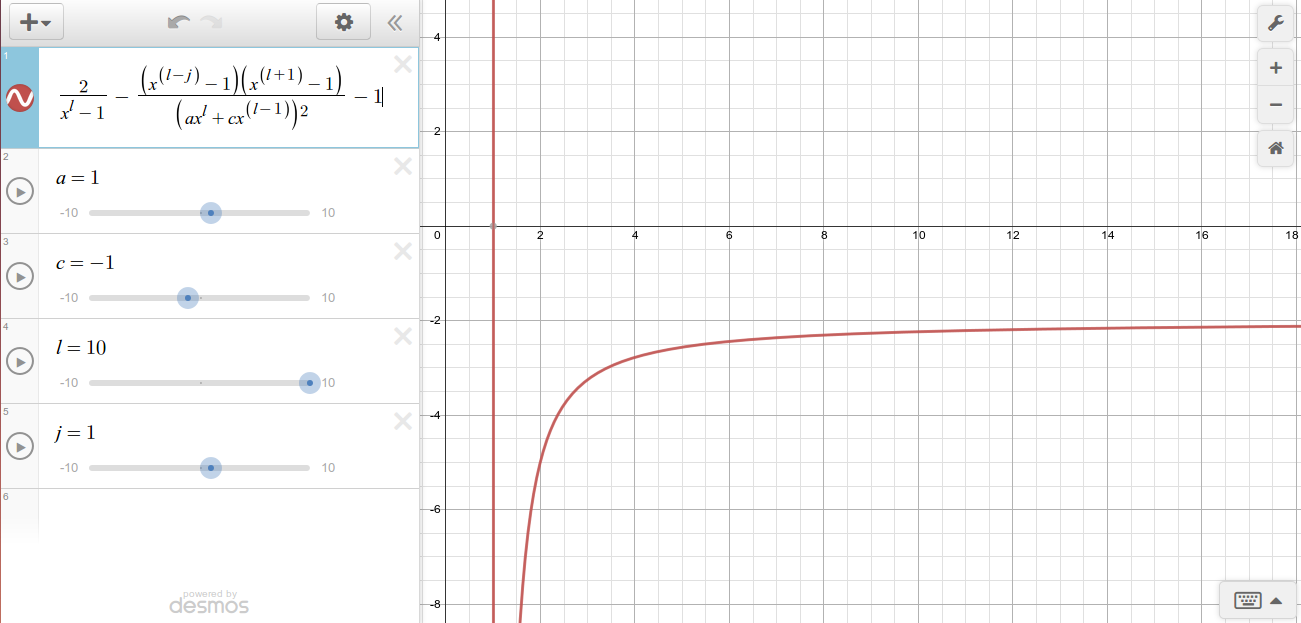
\includegraphics[width=6in]{lower-l10-j1-a1-c1.png}

As you can see, the lower bound difference between our quotient and its approximation is greater than or equal to
$ -2 $ (as our radix grows in size).  We need not worry about real number bounds here because our quotient and its
approximation are integers, and so then is their difference.  Why the choices of $ a=1,\ c=-1 $ ? Of the variations
I looked at, it provided the best bound. In fact when $ a=1 $ and $ c=-1 $ we are assuming the leading digit of
the divisor equals $ b-1 $. This in practice is possible by \emph{normalizing} or scaling both the numerator
and denominator beforehand so that the denominator (divisor) matches this constraint. At the end of the
calculation, we only need remember to scale back.

\begin{verse}
As such the remaining graphs will assume this choice of $ a $ and $ c $ as well.
\end{verse}

The second graph assumes a double digit approximation of a 10 digit divisor with $ a=1 $ and $ c=-1 $:

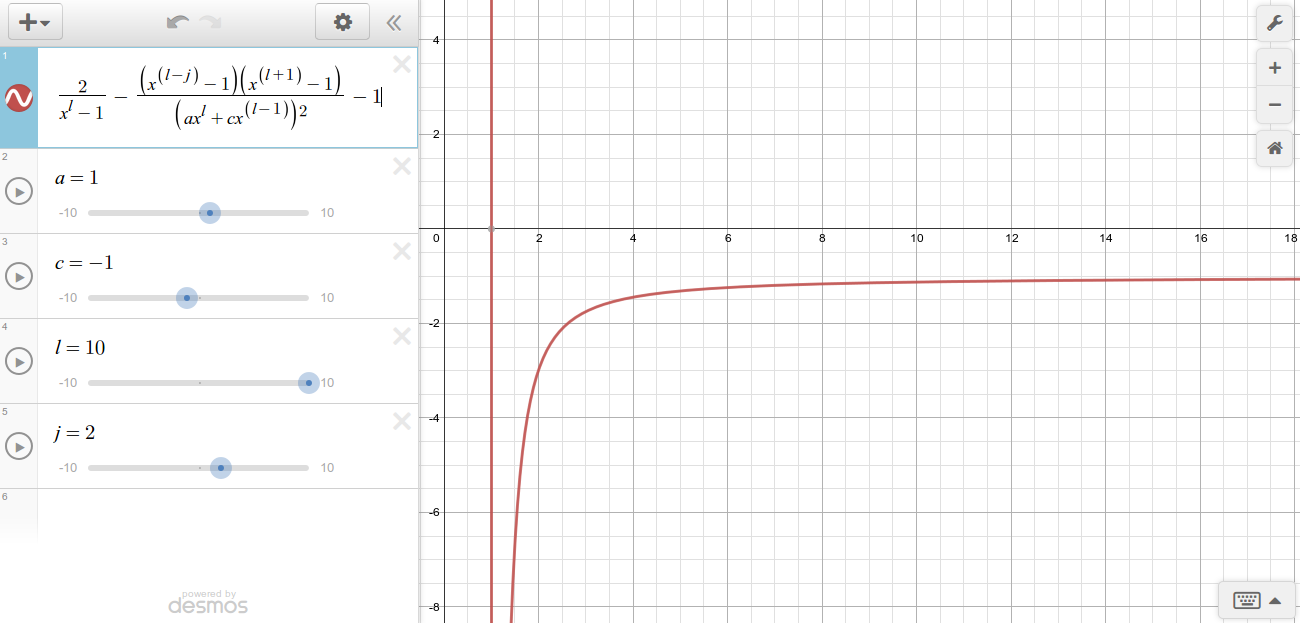
\includegraphics[width=6in]{lower-l10-j2-a1-c1.png}

This might seem redundant as it is similar to the above, but by dividing in two digits we have improved the bound still to $ -1 $.
Is this practical?  Possibly: Our divisor when implemented will be a string of binary, and at the time of writing this the common
architecture is $ 64 $-bit cpu register size. Since we have a division algorithm treating $ 2^{64} $ as our radix (as explained in
the \emph{Single-digit} section), or rather a block of $ 64 $ bits, we can reinterpret our base instead to be $ 2^{32} $ thus
having $ 32 $ bits as our base.  This way, any time we divide by more than half the register length we can assume this improved
bound---meaning less cases to check.

Does it improve efficiency? This much at the time of writing is yet to be determined.

\newpage

Next we look at the upper bound.

We look only at a single digit approximation of a 10 digit divisor with $ a=1 $ and $ c=-1 $:

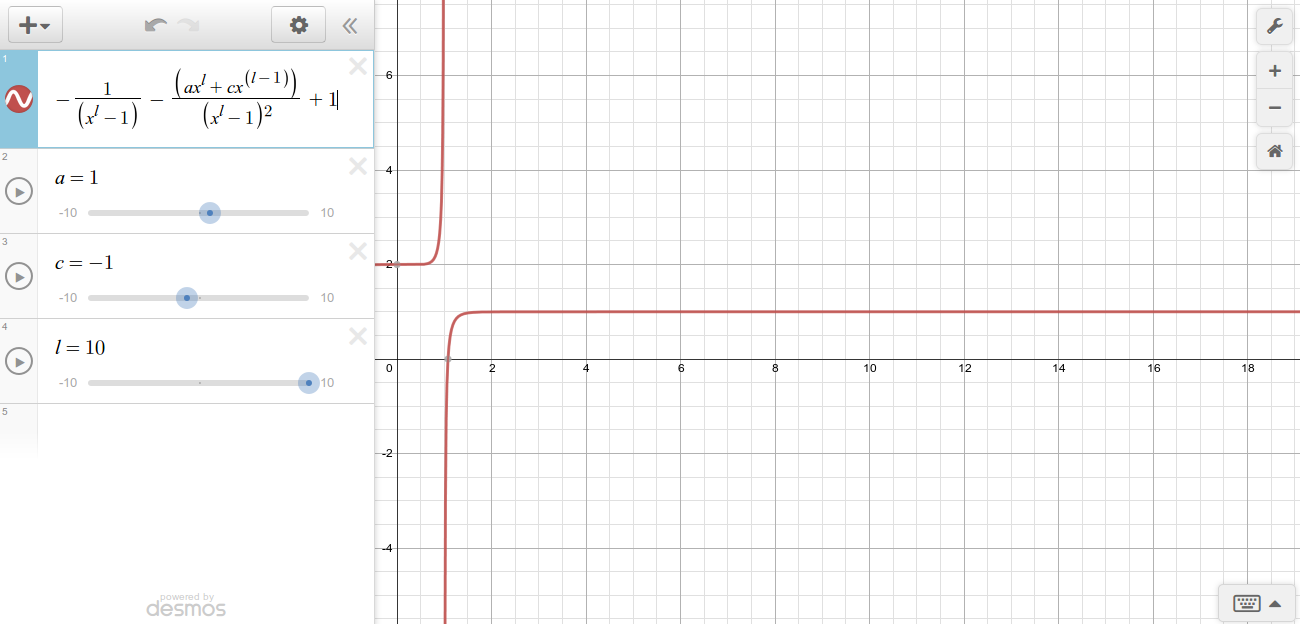
\includegraphics[width=6in]{upper-l10-a1-c1.png}

As you can see, our error term is bounded above by $ 1 $. That's pretty good.\footnote{actually, if you analyze more closely
it converges to $ 1 $ from below, meaning we can do better and round all the way down to $ 0 $, though we won't go so far here.}

Since we've settled upon the constants $ a=1,\ c=-1 $ we need only plug those into our main bound:

$$ \frac{2}{b^\ell-1}-\frac{(b^j-1)(b^{\ell+1}-1)}{(b^\ell-b^{\ell-1})^2}-1
	\leq\left\lfloor\frac{\numer{i}{\ell}}{\denom{i}{\ell}}\right\rfloor
		-\left\lfloor\frac{\numer{j}{\ell}}{\denom{j}{\ell}}\right\rfloor
	\leq-\frac{1}{b^\ell-1}-\frac{b^\ell-b^{\ell-1}}{(b^\ell-1)^2}+1\eqncount $$

For as much effort as we've put into this, it turns out we can do better. Or rather, smarter people
have put in the effort to figure out ways to do better.

\subsection*{The indirect approach: beyond trial and error}

Now onto Knuth's proof.

\subsubsection*{improvements}

Although we haven't proven the following bound (or its required context), our previous intuitive graphs hint at this as a possibility:
$$ -2\leq\left\lfloor\frac{\numer{i}{\ell}}{\denom{i}{\ell}}\right\rfloor
		-\left\lfloor\frac{\numer{j}{\ell}}{\denom{j}{\ell}}\right\rfloor\leq 1 $$

Knuth, says we can do better:
$$ -2\leq\left\lfloor\frac{\numer{i}{\ell}}{\denom{i}{\ell}}\right\rfloor
		-\left\lfloor\frac{\numer{j}{\ell}}{\denom{j}{\ell}}\right\rfloor\leq 0 $$
not only this, but his proof works for \emph{all} radices. If you look at the bounds\footnote{It should be pointed out these
bounds have not actually been proven in this article. It seemed a moot point to otherwise do so as I did not end up using them
in the final proof.} from the intuitive graphs, they only hold for radices greater than or equal to around $ 6 $. This isn't
a problem for our specific application, but it does still mean our previous approach does not provide a universal proof.

How did Knuth come up with this estimate? Inuitively my best guess is since he had access to early day computers, he could have simply
implemented a less efficient version of the division algorithm (as mentioned above) as a baseline to discover inductive evidence toward
a guess. Naturally then he'd still have to prove it, which he did, and that's pretty impressive. It's also possible this result is known
elsewhere in the literature before even his time and he was working on the shoulders of his respective giants, as the saying goes.
Who knows?

Regardless, we are still interested in our error term, and we've already taken the \emph{direct} approach. What's left?
The indirect approach, haha. Knuth uses two separate indirect tricks to derive his lower and upper bounds for the error term.

\newpage

{\bfseries We start with the lower bound.}

This is the more interesting of the two tricks from my viewpoint. The idea is to take advantage of logically equivalent
forms---in particular the \emph{contrapositive} of an implication---as well as the fact that \emph{strict} and \emph{partial}
inequalities are interchangeable when it comes to integers.

Here's what I mean: Let's say you have some interval bound $ e\le x\le f $. With more information, you can always weaken the bound,
which is to say you can derive new bounds in an outwards fashion, say for example we knew that $ d\le e $ and $ f\le g $, then
from the \emph{transitive law} we could easily work outward: $ d\le x\le g $. This was pretty much our direct approach in the
previous subsubsection. On the other hand, it is usually much much harder to work our way inward: To find narrower bounds of $ x $.

As it turns out there is a systematic way to do this. What's the trade off? With the direct approach, we weakened our bounds
by working outward and we did it in order to reduce our dependence upon our central variable(s). The tradeoff here (symmetrically)
is in order to work our way inward we will need to increase our dependence (just a little) upon our central variables.

As stated above, the main trick is to use the contrapositive:
$$ \mbox{If}\qquad A\Longrightarrow B,\quad\mbox{then}\qquad\neg B\Longrightarrow\neg A $$
the rightside of the \emph{then} signifier being read as ``not B implies not A''.

If we were following in Knuth's footsteps, we'd assume in advance we \emph{could} prove that 
$$ -2\leq\left\lfloor\frac{\numer{i}{\ell}}{\denom{i}{\ell}}\right\rfloor
		-\left\lfloor\frac{\numer{j}{\ell}}{\denom{j}{\ell}}\right\rfloor $$
as such, in order to do this we make the contrapositive assumption:
$$ -2\quad >\qquad\left\lfloor\frac{\numer{i}{\ell}}{\denom{i}{\ell}}\right\rfloor
		-\left\lfloor\frac{\numer{j}{\ell}}{\denom{j}{\ell}}\right\rfloor $$
or equivalently
$$ -3\geq\left\lfloor\frac{\numer{i}{\ell}}{\denom{i}{\ell}}\right\rfloor
		-\left\lfloor\frac{\numer{j}{\ell}}{\denom{j}{\ell}}\right\rfloor $$
which we rearrange as
$$ \left\lfloor\frac{\numer{j}{\ell}}{\denom{j}{\ell}}\right\rfloor-3
	\geq\left\lfloor\frac{\numer{i}{\ell}}{\denom{i}{\ell}}\right\rfloor $$
since we're already in contrapostitive mode, we simply work our way outward as before. Here though, it would be ideal if it
were true of the following 
$$ b-1\ge\left\lfloor\frac{\numer{j}{\ell}}{\denom{j}{\ell}}\right\rfloor $$
which seems intuitive enough, but it turns out is \emph{false} in the general context. A simple counterexample such as
$$ \left\lfloor\frac{980}{99}\right\rfloor=9
	\qquad\to\qquad\left\lfloor\frac{98}{9}\right\rfloor=10 $$
demonstrates that we need to take on the additional assumption:
$$ \bar{q}\quad:=\quad\mbox{min}\left(b-1\ ,\ \left\lfloor\frac{\numer{j}{\ell}}{\denom{j}{\ell}}\right\rfloor\right) $$
our $ \bar{q} $ being the same as the notation of Knuth's classical proof, which is defined as our approximation to the
quotient $ q $.  In anycase, we now can say:
$$ b-4\ge\bar{q}-3\ge q $$
or rather
$$ b-4\geq\bar{q}-3
	\geq\left\lfloor\frac{\numer{i}{\ell}}{\denom{i}{\ell}}\right\rfloor $$
of course we will need to do better than this.

Let's take a look at our original approximation:
$$ \left\lfloor\frac{\numer{j}{\ell}}{\denom{j}{\ell}}\right\rfloor $$
we know that
$$ \left\lfloor\frac{\numer{j}{\ell}}{\denom{j}{\ell}}\right\rfloor
	\leq\frac{\numer{j}{\ell}}{\denom{j}{\ell}} $$
but as $ \numer{j}{\ell}\le\numer{i}{\ell} $ this then extends to
$$ \left\lfloor\frac{\numer{j}{\ell}}{\denom{j}{\ell}}\right\rfloor
	\leq\frac{\numer{i}{\ell}}{\denom{j}{\ell}} $$
as well, since $ \denom{i}{\ell}-\denom{j}{\ell}\le b^{j-1}-1 < b^{\ell-1}$,
or rather $ \denom{i}{\ell}-b^{\ell-1} < \denom{j}{\ell} $, we know that
$$ \frac{1}{\denom{j}{\ell}}\quad <\qquad\frac{1}{\denom{i}{\ell}-b^{\ell-1}} $$
and so
$$ \left\lfloor\frac{\numer{j}{\ell}}{\denom{j}{\ell}}\right\rfloor
	\quad <\qquad\frac{\numer{i}{\ell}}{\denom{i}{\ell}-b^{\ell-1}} $$
of course we need to consider the possibility of dividing by zero: $ \denom{i}{\ell}-b^{\ell-1}=0 $. This ends up being
a separate case. Hence the generic proof given here doesn't include it. As for this possibility, our original inequality
claim is that $ \bar{q}-2\le q\le\bar{q} $, which still holds as we in fact more narrowly have equality $ q=\bar{q} $:
$$ \left\lfloor\frac{\numer{i}{\ell}}{b^{\ell-1}}\right\rfloor
	\quad =\quad\left\lfloor\frac{\bseq[w]_{\ell}b^\ell+\bseq[w]_{\ell-1}b^{\ell-1}+\ldots}{b^{\ell-1}}\right\rfloor
	\quad =\quad\left\lfloor\frac{\numer{j}{\ell}}{b^{\ell-1}}\right\rfloor $$

Moving on. With our contrapositive assumption $ 3\le\bar{q}-q $ and the fact that
$$ \frac{\numer{i}{\ell}}{\denom{i}{\ell}}-1\quad <\qquad\left\lfloor\frac{\numer{i}{\ell}}{\denom{i}{\ell}}\right\rfloor=q $$
we have
$$ 3\le\bar{q}-q
	\quad <\qquad\frac{\numer{i}{\ell}}{\denom{i}{\ell}-b^{\ell-1}}-\frac{\numer{i}{\ell}}{\denom{i}{\ell}}+1
	\quad =\qquad\frac{\numer{i}{\ell}}{\denom{i}{\ell}}\left(\frac{b^{\ell-1}}{\denom{i}{\ell}-b^{\ell-1}}\right)+1 $$
which simplifies to
$$ 2\quad <\qquad \frac{\numer{i}{\ell}}{\denom{i}{\ell}}\left(\frac{b^{\ell-1}}{\denom{i}{\ell}-b^{\ell-1}}\right) $$
or rather
$$ 2\left(\frac{\denom{i}{\ell}-b^{\ell-1}}{b^{\ell-1}}\right)\quad <\qquad \frac{\numer{i}{\ell}}{\denom{i}{\ell}} $$
which approximates as
$$ 2\left(\bunderseq[y]{\ell-1}-1\right)
	\leq 2\left(\frac{\denom{i}{\ell}-b^{\ell-1}}{b^{\ell-1}}\right)
	\quad <\qquad \frac{\numer{i}{\ell}}{\denom{i}{\ell}} $$
thus we can finally refine our middle bound of interest
$$ b-4\geq\bar{q}-3
	\geq\left\lfloor\frac{\numer{i}{\ell}}{\denom{i}{\ell}}\right\rfloor $$
to be
$$ b-4\ \ge\ \bar{q}-3\ \ge\ q\ \ge\ 2\left(\bunderseq[y]{\ell-1}-1\right) $$
this implies from the outer range that
$$ b-4\geq 2\left(\bunderseq[y]{\ell-1}-1\right) $$
or rather
$$ \frac{b-4}{2}+1\geq\bunderseq[y]{\ell-1} $$
which simplifies to
$$ \frac{b}{2}-1\geq\bunderseq[y]{\ell-1} $$
and as we started out with a contrapositive, we now negate:
$$ \frac{b}{2}-1\quad <\qquad\bunderseq[y]{\ell-1} $$
which is to say
$$ \left\lfloor\frac{b}{2}\right\rfloor\leq\bunderseq[y]{\ell-1}\qquad\Longrightarrow\qquad -2\le q-\bar{q}\qed $$

{\bfseries Now for the upper bound.}

The trick Knuth uses here is actually to piggyback on the bound of the \emph{division-remainder} theorem itself:

Let $ n,d\in\mathbb{N} $ with $ d > 0 $, then there exist unique $ q, r $ such that
$$ n=qd+r,\qquad 0\le r < d $$

We aim to show now that $ q\le\bar{q} $. As we've added the additional assumption
$$ \bar{q}\quad:=\quad\mbox{min}\left(b-1\ ,\ \left\lfloor\frac{\numer{j}{\ell}}{\denom{j}{\ell}}\right\rfloor\right) $$
we need to consider this possibility as well. For starters, if $ \bar{q}=b-1 $, it is trivially the case that $ q\le\bar{q} $.

Otherwise
$$ \bradix[w]{i\le k\le\ell}-\bar{q}\bradix[y]{i\le k < \ell}
	\leq\bradix[w]{i\le k\le\ell}-\bar{q}\ \bradix[y]{j\le k < \ell} $$
but as $ \bar{q}=\left\lfloor\frac{\numer{j}{\ell}}{\denom{j}{\ell}}\right\rfloor $ we have
$$ \frac{\numer{j}{\ell}+b^j}{\denom{j}{\ell}}-1\le\bar{q} $$
or rather
$$ \bradix[w]{j\le k\le\ell}+b^j-\bradix[y]{j\le k < \ell}\le\bar{q}\bradix[y]{j\le k < \ell} $$
which in a form of more interest to us becomes
$$ -\bar{q}\bradix[y]{j\le k < \ell}\le\bradix[y]{j\le k < \ell}-\bradix[w]{j\le k\le\ell}-b^j $$
adding this back to the above
$$ \begin{array}{rcl}
\bradix[w]{i\le k\le\ell}-\bar{q}\bradix[y]{i\le k < \ell}
	& \leq & \bradix[w]{i\le k\le\ell}+\bradix[y]{j\le k < \ell}-\bradix[w]{j\le k\le\ell}-b^j \\
\\
	& \leq & \bradix[w]{i\le k < j}-b^j+\bradix[y]{j\le k < \ell} \\
\\
	& \quad <\qquad & \bradix[y]{j\le k < \ell}\leq\bradix[y]{i\le k < \ell} \\
\end{array} $$
this would almost be enough to be the complete division-remainder theorem itself and as it states our quotient and remainder
are unique---this would be enough to prove the strong result of equality. Unfortunately, we have no way of proving the lower
bound $ 0\le\numer{i}{\ell}-\bar{q}\denom{i}{\ell} $.

Regardless, what we do have is enough it can be rearranged as
$$ \frac{\numer{i}{\ell}}{\denom{i}{\ell}}
	\quad <\qquad\bar{q}+1 $$
which extends to
$$ q\quad <\qquad\bar{q}+1 $$
which is also known as
$$ q\le\bar{q}\qed $$

\subsubsection*{cleanup}

At this point all we have left are a few cleanup optimizations. Namely, now that we know our approximation
$$ \bar{q}\quad:=\quad\mbox{min}\left(b-1\ ,\ \left\lfloor\frac{\numer{j}{\ell}}{\denom{j}{\ell}}\right\rfloor\right) $$
is such that
$ \bar{q}-2\le q\le\bar{q} $
we are still guessing and checking our quotient, but we've ruled it down to three possibilities. What order do we test these
cases in practice? Is there a faster way to \emph{check} our guess than a full case multiplication? These questions have also
been thought through and answered.

In particular recall in our intuitive graphs when we considered the possibility of dividing by a two digit approximation
our bound narrowed? Here we can use that intuition to optimize our guess and check routine:

$$ \boxed{
\begin{array}{lcccl}
\bar{q} & > & \frac{\numer{\ell-2}{\ell}}{\denom{\ell-2}{\ell}} & \Longrightarrow & q < \bar{q} \\
\\
\bar{q} & \le & \frac{\numer{\ell-2}{\ell}}{\denom{\ell-2}{\ell}} & \Longrightarrow & \bar{q}-1\le q\le\bar{q}
\end{array}
} $$

Starting with
$$ \bar{q}\quad >\qquad\frac{\numer{\ell-2}{\ell}}{\denom{\ell-2}{\ell}} $$
we distribute
$$ \bar{q}\ \bradix[y]{\ell-2\le k < \ell}\quad >\qquad\bradix[w]{\ell-2\le k\le\ell} $$
and extend
$$ \bar{q}\ \bradix[y]{\ell-2\le k < \ell}
	\geq\bradix[w]{\ell-2\le k\le\ell}+b^{\ell-2} $$
then additively invert
$$ -\bar{q}\ \bradix[y]{\ell-2\le k < \ell}
	\leq-\bradix[w]{\ell-2\le k\le\ell}-b^{\ell-2} $$
so similar to our previous ``piggybacking'' proof, we have
$$ \begin{array}{rcl}
\bradix[w]{i\le k\le\ell}-\bar{q}\bradix[y]{i\le k < \ell}
	& \leq & \bradix[w]{i\le k\le\ell}-\bar{q}\bradix[y]{\ell-2\le k < \ell}
\\
	& \leq & \bradix[w]{i\le k\le\ell}-\bradix[w]{\ell-2\le k\le\ell}-b^{\ell-2} \\
\\
	& \leq & \bradix[w]{i\le k < \ell-2}-b^{\ell-2} \\
\\
	& \quad <\qquad & 0 \\
\end{array} $$
this of course implies that
$$ \bradix[w]{i\le k\le\ell}\quad <\qquad\bar{q}\bradix[y]{i\le k < \ell} $$
or rather
$$ \frac{\numer{i}{\ell}}{\denom{i}{\ell}}
	\quad <\qquad\bar{q} $$
which is to say
$$ \left\lfloor\frac{\numer{i}{\ell}}{\denom{i}{\ell}}\right\rfloor
	\quad <\qquad\bar{q}\qed $$
we need not consider the $ \bar{q}=b-1 $ case separately as no restricted assumptions are made in the above.

\newpage

Moving onto
$$ \bar{q}\leq\frac{\numer{\ell-2}{\ell}}{\denom{\ell-2}{\ell}} $$

Given that
$$ \bar{q}\quad:=\quad\mbox{min}\left(b-1\ ,\ \left\lfloor\frac{\numer{\ell-1}{\ell}}{\denom{\ell-1}{\ell}}\right\rfloor\right) $$
let's first consider the case $ \bar{q}=\left\lfloor\frac{\numer{\ell-1}{\ell}}{\denom{\ell-1}{\ell}}\right\rfloor $.

If
$$ \bar{q}\leq\frac{\numer{\ell-2}{\ell}}{\denom{\ell-2}{\ell}} $$
then
$$ 0\leq\bradix[w]{\ell-2\le k\le\ell}-\bar{q}\bradix[y]{\ell-2\le k < \ell} $$

Notice though, similar to an earlier derivation:
$$ \bradix[w]{\ell-2\le k\le\ell}-\bar{q}\bradix[y]{\ell-2\le k < \ell}
	\leq\bradix[w]{\ell-2\le k\le\ell}-\bar{q}\ \bradix[y]{\ell-1\le k < \ell} $$
but as $ \bar{q}=\left\lfloor\frac{\numer{\ell-1}{\ell}}{\denom{\ell-1}{\ell}}\right\rfloor $ we have
$$ \frac{\numer{\ell-1}{\ell}+b^j}{\denom{\ell-1}{\ell}}-1\le\bar{q} $$
or rather
$$ \bradix[w]{\ell-1\le k\le\ell}+b^j-\bradix[y]{\ell-1\le k < \ell}\le\bar{q}\bradix[y]{\ell-1\le k < \ell} $$
which in a form of more interest to us becomes
$$ -\bar{q}\bradix[y]{\ell-1\le k < \ell}\le\bradix[y]{\ell-1\le k < \ell}-\bradix[w]{\ell-1\le k\le\ell}-b^j $$
adding this back to the above
$$ \begin{array}{rcl}
\bradix[w]{\ell-2\le k\le\ell}-\bar{q}\bradix[y]{\ell-2\le k < \ell}
	& \leq & \bradix[w]{\ell-2\le k\le\ell}+\bradix[y]{\ell-1\le k < \ell}-\bradix[w]{\ell-1\le k\le\ell}-b^j \\
\\
	& \leq & \bradix[w]{\ell-2\le k < \ell-1}-b^j+\bradix[y]{\ell-1\le k < \ell} \\
\\
	& \quad <\qquad & \bradix[y]{\ell-1\le k < \ell}\leq\bradix[y]{\ell-2\le k < \ell} \\
\end{array} $$
this is to say:
$$ 0\leq\bradix[w]{\ell-2\le k\le\ell}-\bar{q}\bradix[y]{\ell-2\le k < \ell}
	\leq\bradix[y]{\ell-2\le k < \ell} $$
which by the \emph{uniqueness} of quotient and remainder within the division-remainder theorem automatically implies
$$ \bar{q}=\left\lfloor\frac{\numer{\ell-2}{\ell}}{\denom{\ell-2}{\ell}}\right\rfloor $$
or for our purposes provides us with
$$ \frac{\numer{\ell-2}{\ell}}{\denom{\ell-2}{\ell}}-1\quad <\qquad\bar{q} $$

Regardless of the exact value of $ \bar{q} $ itself, it's fair to say at least:
$$ \bar{q}\le b-1 $$
Also, it has been otherwise assumed:
$$ 2\le b $$
and so
$$ 2\bar{q}\leq (b-1)b $$
putting this and the above together:
$$ \frac{\numer{\ell-2}{\ell}}{\denom{\ell-2}{\ell}}-1
	\quad <\qquad\bar{q}
	\leq \frac{b-1}{2}b
	\leq\frac{\denom{\ell-2}{\ell}}{b^{\ell-2}} $$
Restating this
$$ \frac{\numer{\ell-2}{\ell}}{\denom{\ell-2}{\ell}}
	\quad <\qquad \frac{\denom{\ell-2}{\ell}+b^{\ell-2}}{b^{\ell-2}} $$
Restating this again
$$ \frac{\numer{\ell-2}{\ell}}{\denom{\ell-2}{\ell}}\frac{b^{\ell-2}}{\denom{\ell-2}{\ell}+b^{\ell-2}}
	\quad <\qquad 1 $$
which when decomposed leads us to
$$ \frac{\numer{\ell-2}{\ell}}{\denom{\ell-2}{\ell}}-\frac{\numer{\ell-2}{\ell}}{\denom{\ell-2}{\ell}+b^{\ell-2}}
	\quad <\qquad 1 $$
and by rearranging we get
$$ \frac{\numer{\ell-2}{\ell}}{\denom{\ell-2}{\ell}}
	\quad <\qquad\frac{\numer{\ell-2}{\ell}}{\denom{\ell-2}{\ell}+b^{\ell-2}}+1
	\leq\frac{\numer{i}{\ell}}{\denom{i}{\ell}}+1
	\quad <\qquad q+2 $$
this of course implies
$$ \bar{q} < q+2 $$
or rather
$$ \bar{q}-1\le q\qed $$
It goes without proving that
$$ \bar{q}-1\le q\le\bar{q} $$
though we need still consider the case that $ \bar{q}=b-1 $.

$$ \begin{array}{rcl}
0 & \le & b-2 \\
0 & \le & (b-2)^2 \\
0 & \le & b^2-4b+4 \\
\end{array} $$
but also, $ 0\le b $, so adding these together
$$ 0\quad\le\quad b^2-3b+4 $$
Now, rearranging, seperating, and factoring:
$$ \begin{array}{rcl}
-b^2+2b+2b-4 & \le & b \\
b^3-2b^2-b^2+2b+2b-4 & \le & b^3-2b^2+b \\
(b-2)b^2-(b-2)b+(b-2)2 & \le & (b^2-2b+1)b \\
(b-2)[b^2-b+2] & \le & (b-1)^2b \\
\end{array} $$
and so
$$ \frac{(b-2)[(b-1)b+2]}{(b-1)b}\leq b-1=\bar{q}\leq\frac{\numer{\ell-2}{\ell}}{\denom{\ell-2}{\ell}} $$
now
$$ \begin{array}{rcl}
b-2 & \le & \frac{\numer{\ell-2}{\ell}}{\denom{\ell-2}{\ell}}\frac{(b-1)b}{(b-1)b+2} \\
\\
	& \le & \frac{\numer{\ell-2}{\ell}}{\denom{\ell-2}{\ell}}\left(1-\frac{2}{(b-1)b+2}\right) \\
\end{array} $$

Our interest now becomes:
$$ \frac{2}{(b-1)b+2} $$
first recall
$$ \frac{b-1}{2}b^{\ell-1}\leq\bradix[y]{\ell-2\le k < \ell} $$
and so
$$ \frac{b-1}{2}b\leq\frac{\denom{\ell-2}{\ell}}{b^{\ell-2}} $$
shifting
$$ \frac{b-1}{2}b+1\leq\frac{\denom{\ell-2}{\ell}}{b^{\ell-2}}+1 $$
and simplifying
$$ \frac{(b-1)b+2}{2}\leq\frac{\denom{\ell-2}{\ell}+b^{\ell-2}}{b^{\ell-2}} $$
or rather
$$ \frac{b^{\ell-2}}{\denom{\ell-2}{\ell}+b^{\ell-2}}\leq\frac{2}{(b-1)b+2} $$
and of course additively inverting
$$ -\frac{2}{(b-1)b+2}\leq-\frac{b^{\ell-2}}{\denom{\ell-2}{\ell}+b^{\ell-2}} $$
allows us to continue
$$ \begin{array}{rcl}
	& \le & \frac{\numer{\ell-2}{\ell}}{\denom{\ell-2}{\ell}}\left(1-\frac{2}{(b-1)b+2}\right) \\
\\
	& \le & \frac{\numer{\ell-2}{\ell}}{\denom{\ell-2}{\ell}}\left(1-\frac{b^{\ell-2}}{\denom{\ell-2}{\ell}+b^{\ell-2}}\right) \\
\\
	& \le & \frac{\numer{\ell-2}{\ell}}{\textcolor{blue}{\denom{\ell-2}{\ell}}}
		\frac{\textcolor{blue}{\denom{\ell-2}{\ell}}}{\denom{\ell-2}{\ell}+b^{\ell-2}} \\
\\
	& \le & \frac{\numer{\ell-2}{\ell}}{\denom{\ell-2}{\ell}+b^{\ell-2}} \\
\\
	& \le & \frac{\numer{i}{\ell}}{\denom{i}{\ell}}\quad <\quad q+1 \\
\end{array} $$
from this, as we started with $ b-2 $ and ended with $ q+1 $, we deduce
$$ b-2\quad < \quad q+1 $$
or rather
$$ b-1\quad < \quad q+2 $$
or rather again
$$ \bar{q} < q+2\qed $$

\subsection*{psuedocode}

I'll end all of this with a natural language description of our multiple-digit division algorithm and its optimizations.

\begin{enumerate}
\item If our denominator equals $ 0 $ return an error.
\item If our denominator is greater than our numerator, return $ 0 $.
\item If our denominator equals $ 1 $, return the numerator.
\item If our denominator equals $ 2 $, right shift the numerator as it is a much more efficient subroutine.
\item If our denominator is otherwise a single digit (with respect to our fixed radix), use the single digit implementation.
\item If our denominator is otherwise more than a single digit (with respect to our fixed radix), use the multiple digit implementation.
\end{enumerate}

\newpage

That's pretty basic, and I don't intend to provide psuedocode\footnote{quasi-psuedocode in fact, as it is much more natural language
oriented.} for the single digit implementation, but our multiple digit implementation is sufficiently complex it's worth summarizing here:

\begin{enumerate}
\item Starting with our input
$$ \bradix[x]{0\le k < m}\quad\div\quad\bradix[z]{0\le k < \ell}\qquad,\qquad \ell\le m $$
we first normalize such that the significant digit of our divisor is greater than or equal to
$$ \left\lfloor\frac{b}{2}\right\rfloor\leq\bunderseq[y]{\ell-1} $$
which is to say---as our implementation is in binary---we \emph{left shift}
$$ \bradix[z]{0\le k < \ell}\to\bradix[y]{0\le k < \ell} $$
such that its leftmost digit becomes $ 1 $ (if it is not already). We also left shift
$$ \bradix[x]{0\le k\le m}\to\bradix[w]{0\le k\le m} $$
by the same amount---notice here though that the numerator might incur an additional digit in the process. We can simply assume
the extra digit even if it equals $ 0 $. This of course means we now apply our algorithm to the normalized input
$$ \bradix[w]{0\le k\le m}\quad\div\quad\bradix[y]{0\le k < \ell}\qquad,\qquad \ell\le m $$
\item Our denominator has $ \ell $ digits, as such we compare it to the leading $ \ell $ digits of the numerator. If
$$ \bradix[w]{m-\ell+1\le k\le m}\quad <\qquad\bradix[y]{0\le k < \ell} $$
we add an additional digit
$$ \bradix[w]{m-\ell\le k\le m} $$
if on the other hand
$$ \bradix[w]{m-\ell+1\le k\le m}\geq\bradix[y]{0\le k < \ell} $$
we are already in a position to divide within this step of an otherwise iterative loop.
Either way, let us take the convention that we are now dealing with a partial numerator of the form
$$ \bradix[w]{m-\ell\le k\le m} $$
which fits naturally for the case that we had to add a digit, but in the case that we didn't, let us pretend our leading digit
is now $ 0 $ and the indexing is otherwise decremented by one. This of course is for convenience. We now need to find our single
digit quotient for which we spent so much time and effort optimizing.
\item To find our single digit quotient within this iterative step
$$ q\quad:=\quad\left\lfloor\frac{\numer{m-\ell}{m}}{\denom{0}{\ell}}\right\rfloor $$
we first approximate with our single digit division algorithm:
$$ \bar{q}\quad:=\quad\left\lfloor\frac{\numer{m-1}{m}}{\denom{\ell-1}{\ell}}\right\rfloor $$
if this happens to be such that $ \bar{q}\ge b $, then we set $ \bar{q}:=b-1 $ [this is our $ min(b-1, \ldots) $ constraint].
This test itself can be optimized as we do not need to perform a full division to know in advance if $ \bar{q}\ge b $,
we only need look at their leading digits.  We are now assured our approximation is such that $ \bar{q}-2\le q\le\bar{q} $,
and so we only need test which of these three approximating values $ \{\bar{q}-2, \bar{q}-1, \bar{q}\} $ meets our restriction
$$ 0\leq\bradix[w]{m-1\le k\le m}-q\ \bradix[y]{\ell-1\le k < \ell}\quad <\qquad\bradix[y]{\ell-1\le k < \ell} $$
\item Our test is as follows
$$ \boxed{
\begin{array}{lcccl}
\bar{q} & > & \frac{\numer{m-2}{m}}{\denom{\ell-2}{\ell}} & \Longrightarrow & q < \bar{q} \\
\\
\bar{q} & \le & \frac{\numer{m-2}{m}}{\denom{\ell-2}{\ell}} & \Longrightarrow & \bar{q}-1\le q\le\bar{q}
\end{array}
} $$
So, for example, if
$$ \bar{q}\quad >\qquad\frac{\numer{m-2}{m}}{\denom{\ell-2}{\ell}} $$
then we decrement our $ \bar{q} $, and apply this test again. If it's true again, then we decrement our $ \bar{q} $ again and we
should have our value. Otherwise, if the above relation comes out false (either in the original or in the first decrement),
we know our $ q $ is one of two values, and in this case we have no choice but to do a full multiplication to find out.
Keep in mind our optimized test itself can be implementationally optimized as we can perform it as follows:
$$ \bar{q}\left(\frac{\denom{\ell-2}{\ell}}{b^{\ell-2}}\right)\quad >\qquad\frac{\numer{m-2}{m}}{b^{\ell-2}} $$
which simplifies because our numerator and denominator in this case are both divisible by $ b^{\ell-2} $
(less calculations to perform by theoretically---not computationally---dividing out first) and by changing
its orientation from division to multiplication we will further perform fewer calculations.
\item We now take our known quotient $ q $ and find our remainder
$$ r:=\bradix[w]{m-\ell\le k\le m}-q\ \bradix[y]{0\le k < \ell} $$
which now becomes the new numerator and we go back and repeat this iterative loop in finding the next single digit quotient.
\item Once we have reached a remainder such that $ 0\le r < \denom{\ell-1}{\ell} $ our loop terminates.  We now have all the
necessary quotient digits, and if we are interested in returning the remainder, we right shift this final remainder $ r $ by
the original amount we left shifted our original denominator $ \denom[z]{0}{\ell} $ to reverse our original normalization.

\end{enumerate}

\end{document}

